\title{
	Dojo - Mehr als nur ein Museumsführer
}

\team{
    Dominik Hiltbrunner,
    Tobias Klenke,
    Lattman Emerson,
    Pius Ochs,
    Roman Sonder,
    Alexander Stutz
}

\client{
	Jana Kalbermatter und Hans Gysin
}

\coaches{
    Matthias Meier und Pascal Schleuniger
}

\fssummary{
    Wenn es nach Jana Kalbermatter, einer Absolventin der HGK, geht, sollten 		Museen schon längst modernisiert werden. Ihr letzter Museumsbesuch hat 			gezeigt, dass beim ziellosen umherschweifen Kunstwerke oftmals nicht 			wahrgenommen werden und am Ende nur das Erlebnis ''Besuch'' und nicht 			die Kunstwerke selbst in Erinnernung bleiben. Mit dem Dojo, einem stabförmigen 		Museumsführer soll sich dies nun ändern.
}

\fsgraphics{
    \begin{minipage}{\textwidth}
    	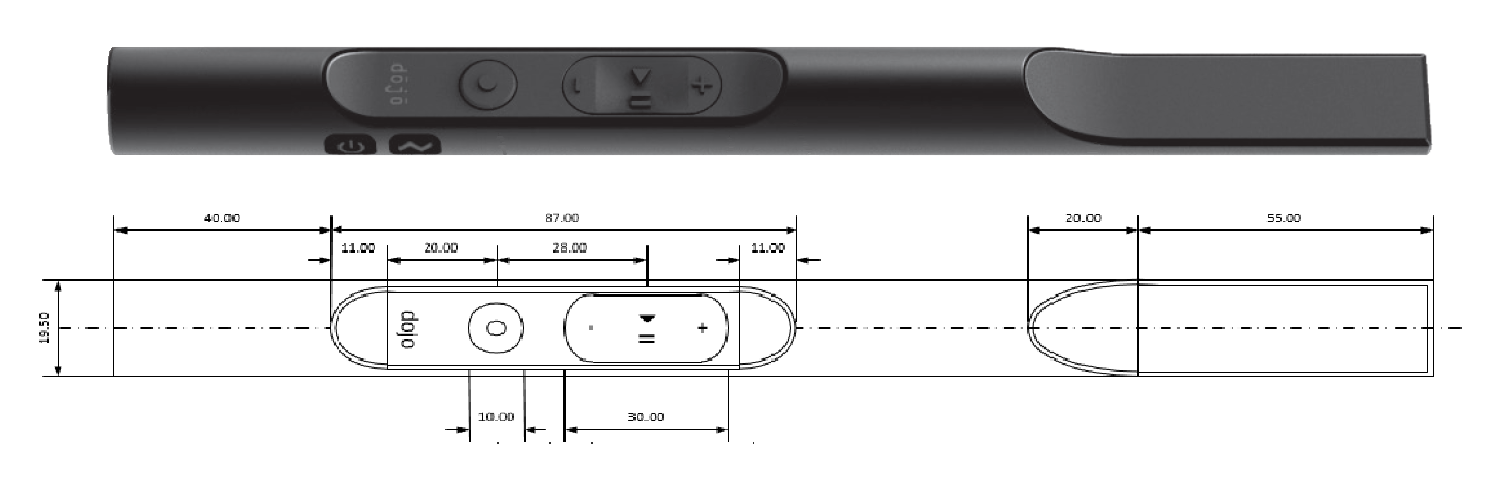
\includegraphics[height=50mm]{graphics/Abbildung_3.png}
        \graphicscaption{	Abbildung 1: Von Auftraggeberin designtes Gehäuse 							mit Dimensionsangaben}
    \end{minipage}
    \graphicssource{Abbildung von Auftraggeberin}
}

\fscontent{
    \section{Die Aufgabe}
    Auf dem Konzept von Jana Kalbermatter beruhend, soll die Elektronik für 		den von Ihr designten Dojo entwickelt werden, welche nicht nur in der 			Lage ist, Kunstwerke im Umfeld zu erkennen und entsprechende 					Audioinformationen bereitzustellen, sondern auch gleich als E-Ticket 			fungieren. Der Dojo soll das Zutrittsrecht zu verschiedenen Räumen 				gewähren können, als auch eine Möglichkeit besitzen, Kunstwerke zu 				''liken''. Beim auschecken kann sodann eine Broschüre als Erinnerung 			mit den ''gelikten'' Kunstwerken bezogen werden. Damit im Museeum auch 			weiterhin Ruhe herrscht, soll die Audioübertragung mittels 						Knochenschallgeber funktionieren.

    \newcol
    
    \section{Die Lösung}
    Mit der entwickelten Elektronik wurde ein erstes Funktionsmodell 				geschaffen, das in der Lage ist, die an Kunstwerken montierten Beacons 			zu erkennen und entsprechende Audioinformationen via Knochenschallgeber 		zur Verfügung zu stellen. Aufgrund der Signalstärken der 						einzelnen Beacons wird entschieden, vor welchem Kunstwerk sich der 				Museumsbesucher befindet und durch Vibration des Dojo eine verfügbare 			Audioinformation angekündigt. Ebenso funktioniert die Zutrittsregelung 			durch bei Drehkreuzen montierten Beacons, welche bei genügender 				Zutrittsberechtigung Zutritt gewähren.

    \section{Die Bedienung}
    Mittels einer mit Java entwickelten Software kann der Dojo mit neuen 			Audioinformationen versorgt, sowie mit vom Besucher gewünschter 				Zutrittsberechtigung und Sprache geladen werden. Anschliessend erhält der 	Besucher den Dojo, der Museumsführer und E-Ticket zugleich. Befindet sich 	der Besucher in Reichweite eines Kunstwerkes, meldet sich der Dojo durch 		Vibration und entsprechende Audioinformationen stehen bereit. Mittels 			''Like-Taste'' kann nun ein Kunstwerk ''geliked'' werden. Beim Abschluss 		des Besuches wird der Dojo zurückgeben, mittels Java Software ausgewertet 	und der Besucher erhält seine persönliche Erinnerungsbroschüre.
}

\infobox{Technische Daten}{
	\begin{tabbing}
		\hspace{40mm}		\= \hspace{15mm} \=\kill
		Gerätebezeichnung:	\> Dojo Museumsführer \\
		Modell:				\> Team 3 \\
		Speicherkapazität:	\> 2 GB \\
		Schnittstelle:		\> USB 2.0 (High Speed) \\
		Abmessungen:		\> ca. 245 mm x 19.5 mm (L x H) \\
		Akku:				\> Wiederaufladbarer Li-Ion Akku; 3.9 V, 600 mAh \\
		Eingang:			\> 5 V, 500 mAh (via USB-Schnittstelle) \\
		Laufzeit*:			\> Bis zu 3 Stunden Abspielzeit \\
\end{tabbing}

\begin{description}
\item *Akkulaufzeit kann je nach Abhängigkeit des Bedienverhaltens variieren.
\end{description}
}
